% Arbeit.tex
% LaTeX-Hauptdatei fuer Studien/Diplomarbeiten am IMMD 9
% geschrieben von Wolfgang Heidrich <wgheidri@immd9.informatik.uni-erlangen.de>
% erweitert von Christian Vogelgsang <cnvogelg@immd9.informatik.uni-erlangen.de>
% und von Darius Rückert <darius.rueckert@fau.de>

% benoetigt LaTeX 2e (z.B. in teTeX)

% --- Style + Optionen ---
% Font: 11pt bevorzugt, 10pt fuer besonders lange Arbeiten.
%       12pt nur in Ausnahmefaellen.
\documentclass[11pt, twoside, openright, a4paper]{studdipl} 

% --- Paketauswahl ---
% a4wide: breites Papierformat
% german: Deutsche Ueberschriften
% epsfig: figures mit EPS Bilder
\usepackage{a4wide}

%\usepackage{biblatex}
\usepackage[
backend=biber,
style=numeric,
bibencoding=utf8,
maxcitenames=1
]{biblatex}
\addbibresource{Literatur.bib}

%%%%%%%%%%%%%%%%%%%%
% nice libraries. Use what you want

\usepackage{graphicx,import}
\usepackage{color}
\usepackage{booktabs}
\usepackage[hidelinks]{hyperref}
\usepackage{todonotes}
\usepackage{siunitx}
\usepackage{amsfonts}	
\usepackage{amsmath}
\usepackage{amssymb}
\usepackage{wrapfig}
\usepackage{multirow}
\usepackage{listings}
\usepackage{algorithmic}
\usepackage[boxed,chapter]{algorithm}
\usepackage{subcaption}
% \caption zb. in \figure wird \small
\usepackage[margin=10pt,font=small,labelfont=bf]{caption}		
\usepackage{pgfplots}
\usepackage{filecontents}
\usepackage{tikz}
\usetikzlibrary{shapes,arrows}
\usetikzlibrary{positioning}
\usetikzlibrary{calc}

\usepackage{acronym}
\usepackage{multicol}
\usepackage{svg}
\usepackage{tabularx}
\usepackage[export]{adjustbox}
\usepackage{mathtools}
\usepackage{xspace}

\newcommand{\FLIP}{\protect\reflectbox{F}LIP\xspace}

\makeatletter
\def\thickhline{%
  \noalign{\ifnum0=`}\fi\hrule \@height \thickarrayrulewidth \futurelet
   \reserved@a\@xthickhline}
\def\@xthickhline{\ifx\reserved@a\thickhline
               \vskip\doublerulesep
               \vskip-\thickarrayrulewidth
             \fi
      \ifnum0=`{\fi}}
\makeatother

\newlength{\thickarrayrulewidth}
\setlength{\thickarrayrulewidth}{2\arrayrulewidth}

\DeclareUnicodeCharacter{02B9}{'}

\newcolumntype{Y}{>{\centering\arraybackslash}X}
% \renewcommand\tabularxcolumn[1]{>{\Centering}m{#1}}
\renewcommand\tabularxcolumn[1]{m{#1}}

\setcounter{biburllcpenalty}{7000}
\setcounter{biburlucpenalty}{8000}

% danke, daniel:
\lstdefinelanguage{CUDA}{morekeywords={
	__device__, __global__, __host__, __constant__, __shared__, __noinline__,
	__syncthreads, __any, pragma, unroll, extern,
	gridDim, blockIdx, blockDim, threadIdx, warpSize,
	min, max, abs, sqrt, exp, pi, pow, log, floor,
	char1, uchar1, char2, uchar2, char3, uchar3, char4, uchar4,
	short1, ushort1, short2, ushort2, short3, ushort3, short4, ushort4,
	int1, uint1, int2, uint2, int3, uint3, int4, uint4,
	long1, ulong1, long2, ulong2, long3, ulong3, long4, ulong4,
	float1, float2, float3, float4, double2, dim3,
	texture, tex1Dfetch, tex1D, tex2D, tex3D,
	cudaReadModeElementType,
	atomicAdd, atomicExch,
	CUresult, CUdevice, CUcontext, CUmodule, CUfunction, CUtexref,
	cuInit, cuDeviceGetCount, cuDeviceGet,
	cuCtxCreate, cuCtxPushCurrent, cuCtxPopCurrent, cuCtxAttach, cuCtxDetach, cuCtxDestroy,
	cuModuleLoad, cuModuleGetFunction,
	cuParamSeti, cuParamSetf, cuParamSetv, cuParamSetSize
}}

\lstdefinelanguage{Scheme}{morekeywords={
	define, begin, if, display, newline, let*, or
}}

% settings for listing environment
\lstset{language=C++,
		alsolanguage=CUDA,
		basicstyle=\small,
		frame=single,
        breaklines=true,
        breakatwhitespace=true,
		numbers=left,
		numberstyle=\tiny,
		xleftmargin=5mm,
		captionpos=b,
		tabsize=4
}

%%%%%%%%%%%%%%%%%%%%

% --- CV Config: ---

% --- weitere Pakete ---

% inputenc: direkte Eingabe von Umlauten erlaubt!
\usepackage[utf8]{inputenc}
% huebsche Rahmen fuer Sourcecodebloecke
\usepackage{fancybox}
\usepackage{bm}

% --- Optionen ---

% steuert das Figure Placement auf den Seiten
\renewcommand{\floatpagefraction}{0.8}

% definiert die Kopfzeile
\lhead[]{\fancyplain{}{\rightmark}}
\rhead[{\fancyplain{}{\leftmark}}]{}

% --- CV Config Ende ---

% Ein wenig liberalere spacing rules
\frenchspacing

\DeclareRobustCommand{\uvec}[1]{{%
		\ifcsname uvec#1\endcsname
		\csname uvec#1\endcsname
		\else
		\bm{\hat{\mathbf{#1}}}%
		\fi
}}

% Matrix: Capital Letters + Fat
\newcommand{\myMatrix}[1]{\bm{\mathit{#1}}}
% Vector: Small letters + Fat
\newcommand{\myVector}[1]{\bm{\mathit{#1}}}
% Scalars: Small letters + thin


% Erlaube groessere Freiraeume zwischen Woertern.
% (wichtig fuer Deutsche Texte wegen der grossen durchschnittlichen
% Wortlaenge). Fuer Englische Arbeiten moeglicherweise weglassen.
% \sloppy

\graphicspath{{../images/}}

% -------------- Konfiguration ------------------------------------------------

\thesistype{Master's Thesis}

% Titel der Arbeit
\title{Filtered Volumetric Representations of Surface Meshes for LOD Rendering}

% AutorIn <- Dein Name :-)
\author{Frederik Böhm}

% Dein Geburtsdatum
\birthday{18. December 1996}

% Dein Geburtsort:
\birthplace{Nuremberg}

% DeinE BetreuerIn:
\supervisor{M. Sc. Nikolai Hofmann}

% Beginn der Arbeit
\bdate{2021/12/15}

% Abgabetermin
\edate{2022/06/15}

% -------------- Ende der Konfiguration ---------------------------------------

\setcounter{secnumdepth}{3}


\begin{document}


% DRAFT MODE
% Erzeugt eine Ueberschrift mit dem Datum des Drafts. Muss fuer die
% endgueltige Version natuerlich auskommentiert werden!!!
\draft

% Der "Vorspann" hat roemische Seitennummern 
\prepages

% short mode: uncomment
% Damit wird die zweite Titelseite erstellt (die erste ist ja in einem
% separaten File)
\maketitle

% eine Leerseite
\cleardoublepage

% Inhaltsverzeichnis
\tableofcontents

\chapter*{Abbreviations}
\begin{acronym}[BRDF]
\acro{lod}[LOD]{Level of Detail}
\acro{brdf}[BRDF]{Bidirectional reflectance distribution function}
\acro{ndf}[NDF]{Normal distribution function}
\acro{vndf}{VNDF}{Distribution of visible normals}
\acro{pdf}[PDF]{Probability density function}
\acro{cdf}[CDF]{Cumulative distribution function}
\end{acronym}
\chapter*{Abstract}
This thesis proposes an approach for \acf{lod} rendering by representing surface meshes with volumes.
We use ray casting to filter the surface meshes and obtain volume representations with differing detail.
The optimal \ac{lod} is selected using a heuristic which compares the number of voxels the camera sees with the number of pixels the volume covers on the image plane.
We test different ratios of these numbers and different minimum voxel sizes in order to find a tradeoff between a good render performance and image quality.
Rendering is done in a custom developed physically based path-tracer.
% \chapter*{Notations}
% \begin{tabular}{ l  l }
%     % \hline
%     % Symbol & Definition \\
%     % \hline
%     $\omega_i$ & Direction from a point of interaction towards the light source \\
%     % \hline
%     $\omega_o$ & Direction from a point of interaction towards the camera \\
%     $\omega_h$ & Half vector: $\omega_h=\frac{\omega_i + \omega_o}{||\omega_i + \omega_o||}$ \\
%     % \hline
%     Bold letters ($\boldsymbol{x}$, $\boldsymbol{y}$, ...) & Points in space \\
%     % \hline
%     $n_{\boldsymbol{x}}$ & The normal at point $\boldsymbol{x}$ \\
%     % \hline
% \end{tabular}

% eine Leerseite
\cleardoublepage
% end of short mode

% der eigentliche Text hat arabische Nummern
\mainbody

% ---------- Kapitel ---------

\chapter{Introduction}
\label{chap:intro}

\section{Motivation}
\label{sect:motivation}

\begin{figure}[!ht]
	\centering
	\includegraphics[width=0.9\linewidth]{image.jpg}
	\caption{caption.}
	\label{img:example}
\end{figure}

\section{Challenges}

\section{Contributions}
 

\chapter{Fundamentals}
This chapter introduces the fundamental concepts necessary for the research.
\section{Surface path-tracing}
We aim to implement a physically based renderer in order to validate the results of our research.
The key property of physically based approaches is the conservation of energy which is given by the rendering equation \cite[p. 1]{rendering_equation}:
\begin{equation}
    \label{eq:render_equation}
    L(\boldsymbol{x}, \omega_o) = L_e(\boldsymbol{x}, \omega_o) + \int_{\mathcal{S}^2} f(\boldsymbol{x}, \omega_o, \omega_i) L(\boldsymbol{y}, -\omega_i) |n_x \cdot w_i| d\omega_i.
\end{equation}
It states that the radiance at a point $x$ in direction $\omega_o$ is given by the emitted radiance at this point plus the integral over the unit sphere $\mathcal{S}^2$ of the \ac{brdf} $f$ times the radiance $L$ coming from $\omega_i$ times the absolute value between the normal $n_x$ at point $x$ and the incident direction $\omega_i$.
Since this equation is in general not analytically solvable we can use Monte Carlo integration to solve it numerically.
For that we have to replace the integral by a sum and divide each summand by the number of summands and by the probability of sampling a direction $\omega_i$ \cite[p. 856]{pbr}:
\begin{equation}
    L(\boldsymbol{x}, \omega_o) = L_e(\boldsymbol{x}, \omega_o) + \frac{1}{N}\sum_{i=1}^{N} \frac{f(\boldsymbol{x}, \omega_o, \omega_i) L(\boldsymbol{y}, -\omega_i) |n_x \cdot w_i|}{p(\omega_i)}.
\end{equation}
The recursive nature of this equation can be observed immediately as we could substitute the radiance $L$ in the sum by the whole equation.
However an implementation in this way is infeasible since that would lead to an exponential growth in the compute time and memory consumption with the recursion depth.
As a solution to this problem \citeauthor{rendering_equation} proposed the \textit{path-tracing} algorithm \cite[p. 6]{rendering_equation}.
Instead of sampling $N$ new directions at each point of intersecting the geometry, we sample a single direction at each intersection point starting at the camera until we hit a light source \cite[p. 6]{rendering_equation}.
This gives us the \textit{path}.
When we repeat this process a large number of times we still get the same result as with using the recursive approach \cite[p. 870]{pbr}.

\section{Volumetric path-tracing}
Since we want to represent our \acsp{lod} by volumes the following chapter introduces how path-tracing can be extended to volumes.
\subsection{Theory of light propagation in participating media}
\label{subsec:theory_of_light_propagation_in_participating_media}
For volumes the radiance along a ray is determined by the in- and out-scattering as well as the emission and absorption properties of the medium \cite[p. 3]{novak_overview}.
\begin{figure}[!ht]
    \centering
    \includegraphics[width=0.8\linewidth]{img/novak_volume_effects.png}
    \caption{The physical effects that are modeled by the \textit{radiative transfer equation} (Image from \cite[p. 2]{novak_overview}).}
    \label{fig:novak_volume_effects}
\end{figure}
The \textit{scattering coefficient} $\mu_s$ and the \textit{absorption coefficient} $\mu_a$ quantify these effects \cite[p. 2]{novak_overview}.
The sum of $\mu_s$ and $\mu_a$ is called the \textit{extinction coefficient} $\mu_t=\mu_a + \mu_s$ and accounts for either of the effects \cite[p. 2]{novak_overview}.
With the integral form of the \textit{radiative transfer equation} we have a way to formalize the scattering, emission and absoption of the medium \cite[p. 3]{novak_overview}:
\begin{equation}
    \label{eq:radiative_transfer}
    L(\boldsymbol{x}, \omega_o) = \int_0^\infty T(\boldsymbol{x}, \boldsymbol{y})[\mu_a(\boldsymbol{y})L_e(\boldsymbol{y}, \omega_o) + \mu_s(\boldsymbol{y})L_s(\boldsymbol{y}, \omega_o)]dy.
\end{equation}
$T$ is the transmittance between point $\boldsymbol{x}$ and point $\boldsymbol{y}$ (Beer-Lambert law) and $L_s$ is the in-scattered radiance which accounts for the radiance scattered into the medium from all directions \cite[p. 3]{novak_overview}:
% \begin{multicols}{2}
% \end{multicols}
% \noindent\begin{minipage}{.5\linewidth}
% \end{minipage}
% \begin{minipage}{.5\linewidth}
% \end{minipage}
\begin{equation}
    \label{eq:beer_lambert_law}
    T(\boldsymbol{x}, \boldsymbol{y}) = e^{-\int_0^y \mu_t(\boldsymbol{x} - s\omega)ds} \;\text{or}\; T(t) = e^{-\int_0^t \mu_t(\boldsymbol{x} - s\omega)ds} \;\text{with}\; t=||\boldsymbol{x}-\boldsymbol{y}||,
\end{equation}
\begin{equation}
    \label{eq:in_scattered_radiance}
    L_s(\boldsymbol{x}, \omega) = \int_{\mathcal{S}^2} f_p(\omega, \omega')L_i(\boldsymbol{x}, \omega')d\omega'.
\end{equation}
$f_p$ is called the \textit{phase function} and will be explained in section \ref{subsec:phase_function}.
Now that we defined how light propagates in a medium, we can combine the formulation in equation \ref{eq:radiative_transfer} with the surface formulation from equation \ref{eq:render_equation}.
We therefore clip the upper integration bound of equation \ref{eq:radiative_transfer} to a distance $z$ and add the surface term \cite[p. 3]{novak_overview}:
\begin{equation}
    L(\boldsymbol{x}, \omega_o) = \int_0^z T(\boldsymbol{x}, \boldsymbol{y})[\mu_a(\boldsymbol{y})L_e(\boldsymbol{y}, \omega_o) + \mu_s(\boldsymbol{y})L_s(\boldsymbol{y}, \omega_o)]dy + T(\boldsymbol{x}, \boldsymbol{z})L(\boldsymbol{z}, \omega_o).
\end{equation}
The idea of this \textit{volume rendering equation} is that a ray passing through a medium will hit a surface at distance $z$ \cite[p. 3]{novak_overview}.
Therefore the radiance $L$ emitted and reflected from this surface is attenuated by the volume transmittance $T$ \cite[p. 889]{pbr}.

\subsection{Solving the Beer-Lambert law in heterogeneous media}
As described in section \ref{subsec:theory_of_light_propagation_in_participating_media} effects like scattering and absoption occur when light interacts with the particles of a medium.
We therefore need a way to sample interactions on which the light than is scattered or absorbed.
On a distance $t=||\boldsymbol{x} - \boldsymbol{y}||$ the Beer-Lambert law from equation \ref{eq:beer_lambert_law} gives us the proportion of light that did not hit a particle $P(X > t) = T(t)$ \cite[p. 5]{novak_overview}.
Therefore we can compute the fraction of light that hit a particle by \cite[p. 5]{novak_overview}
\begin{equation}
    F(t) = 1 - T(t).
\end{equation}
For a homogeneous medium the probability of hitting a particle is therefore
\begin{equation}
    F(t) = 1 - e^{\mu_t t}.
\end{equation}
since $\mu_t$ is constant in the whole medium \cite[p. 5]{novak_overview}.
After rearranging, this gives us a method to sample free path distances in homogeneous media:
\begin{equation}
    \label{eq:distance_sampling}
    t(\xi) = -\frac{ln(1-\xi)}{\mu_t},
\end{equation}
where $\xi$ is a uniform random number in the interval $[0, 1]$ \cite[p. 5]{novak_overview}.

However for heterogeneous media distance sampling is more complex.
We first have to homogenize the medium by adding fictious matter until the extinction reaches the majorant of the real matter $\bar{\mu_t}$ \cite[p. 6]{novak_overview}.
This fictious matter does not influence the scattering or absorption behavior.
We can then iteratively sample new distances using equation \ref{eq:distance_sampling} with $\mu_t=\bar{\mu_t}$ and randomly compare the local extinction coefficient $\mu_t(\boldsymbol{x})$ with the majorant $\bar{\mu_t}$ using a uniform random number $\xi\in[0,1]$ \cite[p. 5]{spectral_and_decomposition_tracking}.
If $\xi<\frac{\mu_t(\boldsymbol{x})}{\bar{\mu_t}}$ we found a hit with a particle and can exit the iteration, if $\xi>=\frac{\mu_t(\boldsymbol{x})}{\bar{\mu_t}}$ we found a null-collision meaning that we have to continue with sampling a new distance $t$ \cite[p. 5]{spectral_and_decomposition_tracking}.
This algorithm is called \textit{delta tracking}.
\begin{figure}[!ht]
    \centering
    \includegraphics[width=0.8\linewidth]{img/novak_delta_tracking.png}
    \caption{For delta tracking we add fictious matter (red circles) to obtain a homogeneous medium (Image from \cite[p. 6]{novak_overview}).}
    \label{fig:novak_delta_tracking}
\end{figure}
To estimate the transmittance in a heterogeneous medium we employ a similar algorithm called \textit{ratio tracking} \cite{novak_ratio_tracking}.
As opposed to delta tracking, ratio tracking does not compare whether the interaction is a null-collision \cite[p. 4]{novak_ratio_tracking}.
Instead it updates the transmission with $T_{new} = T_{old}(1 - \frac{\mu_t(\boldsymbol{x})}{\bar{\mu_t}})$ \cite[p. 4]{novak_ratio_tracking}.

Since both algorithms use a global majorant of the extinction they perform poorly in media where the extinction varies strongly across the medium.
Therefore we use local majorants as suggested in the paper \citetitle{brick_grid} by \citeauthor{brick_grid} \cite{brick_grid}.
\begin{figure}[!ht]
    \centering
    \includegraphics[width=0.9\linewidth]{img/brick_grid_majorants.png}
    \caption{Visualization of the concept of local majorants. These allow to sample distances and estimate transmittance more efficiently (Image from \cite[p. 3]{brick_grid}).}
    \label{fig:brick_grid_datastructure}
\end{figure}
To store the volume data we use three textures.
First we use an \textit{atlas texture} to store \textit{bricks} which are groups of $8 \times 8 \times 8$ voxels \cite[p. 4]{brick_grid}.
The second texture is the \textit{indirection texture} which stores offsets into the atlas.
This texture therefore links a position in space to a brick of data in the atlas \cite[p. 4]{brick_grid}.
Finally we store the minorant and majorant of each brick in the \textit{range texture} \cite[p. 4]{brick_grid}.
These are used to scale the density values in the atlas texture to the interval $[0, 1]$ \cite[p. 4]{brick_grid}.
The range texture additionally has three mipmap levels which allows to have local majorants at different scales \cite[p. 7]{brick_grid}.
\begin{figure}[!ht]
    \centering
    \includegraphics[width=0.9\linewidth]{img/brick_grid_datastructure.png}
    \caption{Datastructure of brick grid (Image from \cite[p. 4]{brick_grid}).}
    \label{fig:brick_grid_datastructure}
\end{figure}
Since the resulting atlas texture no longer has spatial coherence, hardware interpolation by the texture unit is not possible \cite[p. 5]{brick_grid}.
Therefore we employ a form of stochastic lookup where we jitter the lookup point by $\pm0.5$ voxels before doing point sampling \cite[p. 5]{brick_grid}.
When having a large number of lookups, as it is the case in Monte Carlo integration, this is equivalent to trilinear interpolation without introducing a significant overhead \cite[p. 5]{brick_grid}.

For distance sampling and transmittance estimation we first sample a target optical thickness $\tau_{target}=-ln(1-\xi)$ \cite[p. 6]{brick_grid}.
We then accumulate the optical thicknesses of all bricks along a ray until the accumulated thickness exceeds the target thickness \cite[p. 6]{brick_grid}.
In this case we step back along the ray until it matches $\tau_{target}$ \cite[p. 6]{brick_grid}.
Now we perform the stochastical null-collision test by comparing the density at this point with the local majorant \cite[p. 6]{brick_grid}.
In the case of distance sampling, we return the distance to the first real collision \cite[p. 6]{brick_grid}.
For transmittance estimation, we adjust the current estimate by the ratio of real to fictious matter \cite[p. 6]{brick_grid}.
When having a null-collision, the algorithm is restarted by sampling a new target optical thickness \cite[p. 6]{brick_grid}.
This is repeated until a distance is successfully sampled, the transmittance estimation is ended by russian roulette or when the ray left the volume \cite[p. 6]{brick_grid}.

\subsection{Phase functions}
\label{subsec:phase_function}
Equation \ref{eq:in_scattered_radiance} already used the term of a \textit{phase function}, now we want to explain this concept in more detail.
Similar like a \acs{brdf} gives the amount of light scattered into a certain direction on a surface, a phase function gives this amount in a volume \cite[p. 2]{novak_overview}.
The simplest phase function possible is an isotropic phase function in the form
\begin{equation}
    f_p(\omega, \omega')=\frac{1}{4\pi}.
\end{equation}
As it can be seen it has a constant value for all directions $\omega$, $\omega'$ on the unit sphere \cite[p. 2]{novak_overview}.
% TODO: Edit w_o and w_i
\section{\citefield{sggx}{title}}
Since we represent our \acp{lod} as volumes choosing a phase function is required to compute the scattering directions in the medium.
We choose the SGGX phase function because it has similar scattering properties as the GGX \ac{brdf}\cite[p. 2]{sggx}.
The idea behind the GGX \ac{brdf} and other microfacet models is that a surface can be modeled by a distribution of normals which describe the roughness of the surface at a certain point \cite[p. 3]{ggx}.
Expanding on this idea \citeauthor{microflake} introduced the microflake framework which models the medium as two-sided specularly reflecting flakes which are distributed according to a certain \ac{ndf} \cite[pp. 4-5]{microflake}.
\citeauthor{sggx} define the \ac{ndf} for the SGGX phase function as:
\begin{equation}
    D(\omega_m)=\frac{1}{\pi \sqrt{|S|}(\omega_m^T S^{-1} \omega_m)^2},
\end{equation}
where $\omega_m$ is the direction of the microflake normal and $S$ is a 3 $\times$ 3 symmetric positive definite matrix which encodes the scattering properties \cite[p. 4]{sggx}.
This \ac{ndf} can be seen as the extension of the GGX \acs{ndf} to the negative hemisphere:
\begin{figure}[!ht]
    \centering
    \begin{subfigure}[b]{0.45\linewidth}
        \centering
        \includegraphics[width=\linewidth]{img/sggx_ndf_a.jpg}
        \caption{GGX $D(\omega_m), \omega_m \in \Omega^+$ \cite[p. 3]{sggx}}
        \label{fig:sggx_ndf_a}
    \end{subfigure}
    \begin{subfigure}[b]{0.45\linewidth}
        \centering
        \includegraphics[width=1\linewidth]{img/sggx_ndf_b.jpg}
        \caption{SGGX $D(\omega_m), \omega_m \in \Omega$ \cite[p. 3]{sggx}}
        \label{fig:sggx_ndf_b}
    \end{subfigure}
	\caption{Visualization of anisotropic \acsp{ndf}. Note that the negative hemisphere of the SGGX \acs{ndf} is a mirroring of the positive hemisphere.}
	\label{img:sggx_ndf}
\end{figure}
Based on the \acs{ndf} the authors then introduce a \ac{vndf} $D_{\omega_i}(\omega_m)$ which is used for importance sampling of the phase function, since it reduces variance as opposed to the \acs{ndf} \cite[p. 9]{vndf_importance_sampling}.
Another important concept in the mikroflake framework is the projected area $\sigma(\omega_i)$ of the microflakes.
This is the area of the microflakes when projected onto a plane in direction $\omega_i$ \cite[p. 3]{sggx}.
\begin{figure}[!ht]
    \centering
    \includegraphics[width=0.3\linewidth]{img/sggx_projected_area.png}
    \caption{Projected area $\sigma(\omega_i)$ \cite[p. 2]{sggx}.}
    \label{fig:sggx_projected_area}
\end{figure}
For the SGGX phase function the projected area is defined as \cite[p. 4]{sggx}:
\begin{equation}
    \label{eq:projected_area}
    \sigma(\omega_i)=\int_\Omega \langle \omega_i, \omega_m \rangle D(\omega_m) d\omega_m = \sqrt{\omega_i^T S \omega_i},
\end{equation}
where $\langle -,-\rangle$ denotes the clamped dot product \cite[p. 3]{sggx}.
Having defined these terms the authors introduce the actual phase function which consists of a specular and a diffuse component.
The specular component is evaluated as \cite[p.7]{sggx}:
\begin{equation}
    f{}^{spec}_p(\omega_i \rightarrow \omega_o) = \frac{D(\omega_h)}{4 \sigma(\omega_i)}.
\end{equation}
Importance sampling the specular component requires to sample a normal from $D_{\omega_i}$ and the direction $\omega_i$ is reflected on this normal to generate an outgoing direction $\omega_o$ \cite[p. 8]{sggx}.
For evaluating the diffuse phase function \citeauthor{sggx} propose to sample a normal $\omega_m$ from $D_{w_i}$ which gives an unbiased estimate of the following integral \cite[p. 8]{sggx}:
\begin{equation}
    f{}^{diff}_p(\omega_i \rightarrow \omega_o) = \frac{1}{\pi}\int_\Omega \langle\omega_o,\omega_m\rangle D_{\omega_i}(\omega_m) d\omega_m = \lim \limits_{N \to +\infty} \frac{1}{N} \sum_{n=1}^N \frac{1}{\pi} \langle\omega_o,\omega_m(n)\rangle.
\end{equation}
$f{}^{diff}_p$ can then be importance sampled by generating a direction $\omega_m$ from $D_{\omega_i}$ and then sampling the hemisphere given by $\omega_m$ \cite[p. 8]{sggx}.

\section{\citefield{hybrid_mesh_volume_lods}{title}}
Another important paper for the thesis is \citetitle{hybrid_mesh_volume_lods} by \citeauthor{hybrid_mesh_volume_lods}.
Their idea is to represent macroscopic surfaces (larger than the target resolution) as mesh \acsp{lod} while microscopic geometry (smaller than the target resolution) is represented in volumes \cite[p. 3]{hybrid_mesh_volume_lods}.
This is different to our approach as we represent both cases by volumes.
The first step in their pipeline is to seperate the macroscopic from the microscopic geometry \cite[p. 5]{hybrid_mesh_volume_lods}.
For a tree that would mean to seperate the trunk from the branches and leafs \cite[p. 3]{hybrid_mesh_volume_lods}.
The second step is to apply mesh simplification on the macroscopic surface while preserving the reflectance properties.
They achieve mesh simplification by using edge collapse, therefore they remove triangle edges which are smaller than the target resolution.
The adjacent triangles collapse as a result as well \cite[p. 6]{hybrid_mesh_volume_lods}.
To preserve reflectance the authors update the diffuse and specular albedos of the remaining vertices by a weighted sum of the old vertices \cite[p. 6]{hybrid_mesh_volume_lods}.
The last step in their pipeline is the voxelization of the sub-resolution geometry.
The authors choose a ray casting approach to estimate the density for each voxel \cite[p. 8]{hybrid_mesh_volume_lods}.
To sample ray origins the authors use a \ac{pdf} $D_i=D_i^{cube} \ast D^{smooth}$ around the voxel center \cite[p. 9]{hybrid_mesh_volume_lods}.
$D_i^{cube}$ is a cubic uniform \ac{pdf} around the voxel center and $D^{smooth}$ is a 3D gaussian function with the standard deviation of 0.6 times the length of the voxel edge \cite[p. 9]{hybrid_mesh_volume_lods}.
The length of the rays is set to the length of the voxel edge \cite[p. 9]{hybrid_mesh_volume_lods}.
We deviate from this ray generation procedure as we choose the ray origin on a cubic uniform \ac{pdf} around the voxel center and clip our rays at a bounding sphere around the voxel.
Details to our procedure are explained in section \dots.
Each ray is intersected with the micro-geometry, the number of hits and the total number of rays casted determine the occlusion probability \cite[p. 8]{hybrid_mesh_volume_lods}:
\begin{equation}
    P_{occ}=\frac{nbHits}{nbRays}.
\end{equation}
Since a medium is defined on the density $\rho$ the authors solve the integral
\begin{equation}
    1 - \frac{1}{4\pi}\int_\Omega e^{-\rho\sigma_u(\omega)ray_l} d\omega = P_{occ}
\end{equation}
for $\rho$ \cite[p. 9]{hybrid_mesh_volume_lods}.
$\sigma_u(\omega)$ is the microflake projected area as defined in \ref{eq:projected_area} and $ray_l$ is again the length of the voxel edge.
This equation cannot be solved analytically and therefore requires gradient descent based optimization of $\rho$ \cite[p. 9]{hybrid_mesh_volume_lods}.
In section \dots we further explore this optimization procedure.


 

\chapter{Method}
\label{chap:method}
For our experiments, we follow the steps depicted in Figure \ref{fig:pipeline}.
\begin{figure}[t]
    \centering
    \includegraphics[width=1.0\linewidth]{img/pipeline.png}
    % \includesvg[pretex=\tiny, width=1.0\linewidth]{img/pipeline}
    \caption[Visualization of the pipeline the thesis built upon]{Visualization of our pipeline for \ac{lod} generation. Yellow boxes represent files that are inputs our outputs of green program components. Evaluation is partially done by visual comparison and by computing image quality metrics.}
    \label{fig:pipeline}
\end{figure}
We first take the surface meshes and apply the filtering procedure to obtain the volume grids.
Additionally, we save metadata like the bounding-box sizes of the grids, which we need for scene generation.
This generation step can either generate ground-truth scenes that only contain meshes or it can generate scenes that use \acp{lod}.
We generate the scenes once and store the scene description to disk.
The next step in the pipeline is the rendering of the scene, which uses mesh or volume files depending on the definitions in the generated scene file.
Finally, we evaluate our results by comparing the mesh-only renderings with the ones that use \acsp{lod}.
This is done regarding the image quality, the memory usage and the render performance.
We are not interested in the absolute render times, but rather in the relative times between the mesh and volume representations.
This final evaluation step is explained in Chapter \ref{chap:results_and_discussion}, while all other steps are subject of this chapter.

Although our pipeline can be used with arbitrary models, we only use tree models with it.
Trees generally are difficult to render, which makes them a good benchmark for our approach.
The difficulties stem from the high detailed geometry of the branches and leaves, which can lead to aliasing.
As leaves usually are modeled as simple planes with alpha maps applied to them, they pose another challenge on the isotropic volumes that we use.
The trees that we use are 26 free tree meshes from XfrogPlants \cite{xfrogplants} and the McGuire Computer Graphics Archive \cite{McGuire2017Data} which are available as \texttt{.obj} files with the textures being encoded as \texttt{.png} or \texttt{.tiff}.
Meshes and textures together occupy 1.2 GB of disk memory.
Apart from the models itself, XfrogPlants also provides information of the sizes the trees grow during their lifespan, which we also need during filtering and scene generation.

\section{Mesh Filtering}
\label{sec:mesh_filtering}
As described in Section \ref{sec:transforming_meshes_into_volumes}, we use the ray casting approach by \citeauthor{hybrid_mesh_volume_lods} with a few modifications for our filtering \cite{hybrid_mesh_volume_lods}.
The ray casting is \ac{gpu} accelerated using OptiX \cite{parker_optix}.
In contrast to \citeauthor{hybrid_mesh_volume_lods}, we assume our particles to have an isotropic microflake projected area $\sigma$, meaning that it is not view dependent.
An isotropic projected area implies that the particles are spheres, since a sphere has the same shape from all directions.
If the geometry, that should be represented by an isotropic medium, has a non-spherical shape, an error is introduced.
This error gets largest for planar geometry: A perfect plane is invisible when viewed parallelly, but it is opaque for perpendicular viewing directions.
Despite this shortcoming of isotropic media, we choose them for the \acsp{lod}, because this greatly simplifies our optimization procedure during filtering, as well as the distance sampling and transmittance estimation during rendering.

For filtering, a mesh is scaled to match the tree's natural size that is provided by XfrogPlants \cite{xfrogplants}.
We then place the voxel grid over the mesh and align it to three sides of the bounding box of the mesh.
The number of voxels in the grid is determined from the edge length of a voxel and the size of the mesh's bounding box.
If the edge lengths of the mesh's bounding box do not evenly divide by the size of a voxel, we let the volume overlap on the non-aligned sides.
In each voxel we then sample the origin of our rays on a cubic uniform domain and the direction of the rays is uniformly sampled over the unit sphere.
\citeauthor{hybrid_mesh_volume_lods} use a ray length that is equal to the edge length of a voxel, which leads to blurring since adjacent geometry is included in the density estimation.
As \citeauthor{wang_object_space_aliasing} point out, this can reduce object space aliasing \cite{wang_object_space_aliasing}.
However, we think, that we can increase the spatial resolution while still minimizing object space aliasing by clipping the ray at a bounding sphere.
We position the sphere at the voxel's center and scale it such that its diameter is slightly larger than the diagonal of the voxel.
Each ray is then first intersected with this sphere to compute a $t_{max}$, before intersecting it with the actual geometry.
Figure \ref{fig:raygen_filtering} compares our approach for determining the ray length with the approach of \citeauthor{hybrid_mesh_volume_lods} \cite{hybrid_mesh_volume_lods}.
\begin{figure}[t]
    \centering
    \begin{subfigure}[b]{0.25\linewidth}
        \centering
        \includegraphics[width=\linewidth]{img/raygen_filtering_unclipped.png}
        \caption{}
        \label{fig:raygen_filtering_unclipped}
    \end{subfigure}
    \begin{subfigure}[b]{0.25\linewidth}
        \centering
        \includegraphics[width=1\linewidth]{img/raygen_filtering_clipped.png}
        \caption{}
        \label{fig:raygen_filtering_clipped}
    \end{subfigure}
	\caption[Approaches for determining a ray length for filtering]{Image (a) shows the approach by \citeauthor{hybrid_mesh_volume_lods} \cite{hybrid_mesh_volume_lods} with constant ray length. Figure (b) shows our approach with ray clipping at a bounding sphere.}
	\label{fig:raygen_filtering}
\end{figure}

With these modifications we also have to solve a different integral than that from Equation \ref{eq:loubet_filtering_equation}.
We now have to find a density $\rho$ that suffices:
\begin{equation}
    1 - \frac{1}{4\pi}\int_{\mathcal{S}^2} e^{-\rho \, \sigma \, ray_l(\omega)} d\omega = P_{occ}.
    \label{eq:our_filtering_equation}
\end{equation}
Note that the projected area $\sigma$ is now independent of the direction $\omega$, whereas the ray length depends on $\omega$, since the rays are clipped by the bounding sphere.
If we didn't employ ray clipping, we could solve the integral analytically for the density, but since the ray length depends on the direction $\omega$ we iteratively optimize $\rho$:
\begin{equation*}
    \rho_{i+1}=\rho_i - \gamma (P_{occ,volume} - P_{occ,mesh}),
\end{equation*}
where $i$ denotes the iteration and $\gamma$ is a learning rate.
$P_{occ,mesh}$ is the ratio of geometry hits to the total number of rays casted and $P_{occ,volume}$ is the probability that a medium interaction takes place given the density $\rho_i$.
It is computed by Monte Carlo integrating Equation \ref{eq:our_filtering_equation}, so our estimator has the form:
\begin{equation*}
    1 - \frac{1}{N}\sum_{n=1}^{N} e^{-\rho \, \sigma \, ray_l(\omega_n)} = P_{occ,volume}.
\end{equation*}
Apart from this density estimate we also filter the diffuse and specular color of the geometry, the normals, the index of refraction and the SGGX Matrix $S$ by averaging.
The Matrix $S$ serves as a coordinate frame when sampling the phase function \cite{sggx}.

% In total our attributes occupy 80 bytes of memory per voxel and we first represent them by a dense grid in the \ac{GPU}'s global memory.
We represent these attributes as a dense grid in the \acs{gpu}'s global memory.
OpenVDB cannot be used for this, because it is incompatible with CUDA device code \cite{museth_nanovdb}.
NanoVDB can be used on the \ac{gpu}, but it is a read-only grid \cite{nanovdb}.
Only after copying the dense grid to host memory, we convert it into an OpenVDB grid and subsequently into a NanoVDB grid which we store on disk.
The usage of NanoVDB imposes a limit of storing 32 bytes per voxel \cite{open_to_nanovdb}, but our attributes occupy 80 bytes of memory.
Increasing this limit results in a major implementation overhead, so we use quantization to compress the values in the grid.
Before doing computations like interpolation or shading, we transform them back to the full width.
The following table summarizes the size of all attributes in regular and quantized format (ignoring padding):
\begin{center}
    \begin{tabular}{| c | c | c | }
        \hline
         & Regular Format & Quantized Format \\
         \hline
         Density & $1\times 4\;\text{bytes}$ & $1\times 4\;\text{bytes}$ \\
         \hline
         $S$ & $9\times 4\;\text{bytes}$ & $6\times 2\;\text{bytes}$ \\
         \hline
         Diffuse color & $3\times 4\;\text{bytes}$ & $3\times 1\;\text{bytes}$ \\
         \hline
         Specular color & $3\times 4\;\text{bytes}$ & $3\times 1\;\text{bytes}$ \\
         \hline
         Normal & $3\times 4\;\text{bytes}$ & $3\times 2\;\text{bytes}$ \\
         \hline
         Index of refraction & $1\times 4\;\text{bytes}$ & $1\times 2\;\text{bytes}$ \\
         \thickhline
         Total & $80\;\text{bytes}$ & $30\;\text{bytes}$ \\
         \hline
    \end{tabular}
\end{center}
Note that since $S$ is a symmetric matrix, it is enough to store six coefficients \cite{sggx}.
Apart from storing the NanoVDB grid, we also store the brick grid, which only contains the density values of each voxel.
In principle, it would be possible to store all voxel attributes in the brick grid, though the expected performance gain would not have been worth the implementation overhead.
The lower cache coherency of using two grids only has a small impact on the performance, since we use the NanoVDB grid only after having sampled a collision with the brick grid.
Besides the two grids, we also export metadata for every \ac{lod}, which encompasses the number of voxels in the grid, the positions of the eight bounding-box vertices and the bounding box dimensions during filtering.

We generate 7 \acsp{lod} for voxel sizes from $\SI{0.1}{\m}$ to $\SI{6.4}{\m}$, doubling the size of a voxel for each \ac{lod}.
The number of voxels is then computed from the voxel size and the size of the mesh.
We settled for these voxel sizes, as for smaller voxels the grid quickly exceeds the mesh representation in terms of memory consumption.
Choosing even larger sizes has no effect, since some trees are already represented by a single voxel on the coarsest level.
We cast 100 rays in each voxel to estimate the occlusion probability and optimize the density $\rho$ in 20 iterations. % TODO: Discuss dynamic number of rays depending on voxel size
On average it takes $\SI{0.14}{\s}$ to filter a model and the resulting grids of all models occupy 940 MB of disk space, which is 260 MB less than what the mesh representations need.
The finest \acsp{lod} are responsible for 65\% of the occupied disk space.
In Chapter \ref{chap:results_and_discussion} we discuss how dropping this \ac{lod} affects image quality and rendering times.

% Having the \acsp{lod}, Figure \ref{fig:lods_comparison} compares them to the surface representation for some models.
% A comparison for some models between two \acsp{lod} and the corresponding surface representation is illustrated in Figure \ref{fig:lods_comparison}.
For a few selected models, we compare two of their \acsp{lod} with the surface representation in Figure \ref{fig:lods_comparison}.
\begin{figure}[t]
    \begin{center}
        \begin{minipage}[c]{0.24\textwidth}
            \begin{flushleft}
                Model
            \end{flushleft}
        \end{minipage}
        \begin{minipage}[c]{0.24\textwidth}
            \centering
            Mesh
        \end{minipage}
        \begin{minipage}[c]{0.24\textwidth}
            \centering
            Volume \\ (Voxel size = 0.1m)
        \end{minipage}
        \begin{minipage}[c]{0.24\textwidth}
            \centering
            Volume \\ (Voxel size = 0.8m)
        \end{minipage}
    
        \begin{minipage}[c]{0.24\textwidth}
            \begin{flushleft}
                Acer rubrum adult \\
                (Height = $\SI{20.5}{\m}$)
            \end{flushleft}
        \end{minipage}
        \begin{minipage}[c]{0.24\textwidth}
            \includegraphics[valign=c, width=\linewidth]{img/EA01a_mesh.png}
        \end{minipage}
        \begin{minipage}[c]{0.24\textwidth}
            \includegraphics[valign=c, width=\linewidth]{img/EA01a_0.1.png}
        \end{minipage}
        \begin{minipage}[c]{0.24\textwidth}
            \includegraphics[valign=c, width=\linewidth]{img/EA01a_0.8.png}
        \end{minipage}
    
        \begin{minipage}[c]{0.24\textwidth}
            \begin{flushleft}
                Acacia sophorae 9 \\
                (Height = $\SI{8}{\m}$)
            \end{flushleft}
        \end{minipage}
        \begin{minipage}[c]{0.24\textwidth}
            \includegraphics[valign=c, width=\linewidth]{img/OC41_9_mesh.png}
        \end{minipage}
        \begin{minipage}[c]{0.24\textwidth}
            \includegraphics[valign=c, width=\linewidth]{img/OC41_9_0.1.png}
        \end{minipage}
        \begin{minipage}[c]{0.24\textwidth}
            \includegraphics[valign=c, width=\linewidth]{img/OC41_9_0.8.png}
        \end{minipage}
    
        \begin{minipage}[c]{0.24\textwidth}
            \begin{flushleft}
                Celtis australis medium \\
                (Height = $\SI{9.5}{\m}$)
            \end{flushleft}
        \end{minipage}
        \begin{minipage}[c]{0.24\textwidth}
            \includegraphics[valign=c, width=\linewidth]{img/EU06m_mesh.png}
        \end{minipage}
        \begin{minipage}[c]{0.24\textwidth}
            \includegraphics[valign=c, width=\linewidth]{img/EU06m_0.1.png}
        \end{minipage}
        \begin{minipage}[c]{0.24\textwidth}
            \includegraphics[valign=c, width=\linewidth]{img/EU06m_0.8.png}
        \end{minipage}
    
        \begin{minipage}[c]{0.24\textwidth}
            \begin{flushleft}
                Pinus muricata adult \\
                (Height = $\SI{20}{\m}$)
            \end{flushleft}
        \end{minipage}
        \begin{minipage}[c]{0.24\textwidth}
            \includegraphics[valign=c, width=\linewidth]{img/CL13a_mesh.png}
        \end{minipage}
        \begin{minipage}[c]{0.24\textwidth}
            \includegraphics[valign=c, width=\linewidth]{img/CL13a_0.1.png}
        \end{minipage}
        \begin{minipage}[c]{0.24\textwidth}
            \includegraphics[valign=c, width=\linewidth]{img/CL13a_0.8.png}
        \end{minipage}
    \end{center}
    \caption[Comparison between mesh and volume renderings]{Comparison between the surface representation in the first column, the \ac{lod} with a voxel size of $\SI{0.1}{\m}$ in column two and the \ac{lod} with a voxel size of $\SI{0.8}{\m}$ in the last column. The heights of the trees are taken from XfrogPlants \cite{xfrogplants}.}
    \label{fig:lods_comparison}
\end{figure}

\section{Scene Generation}
\label{sec:scene_generation}
We implement the scene generator in Python.
It uses the volume metadata that is exported during filtering and generates a circular forest region with uniformly distributed trees.
Our generator uses a rejection sampling approach, rejecting samples that are too close to another.
It is similar to a Poisson disk sampler \cite{poisson_sampling}, however it uses varying spacing between the samples depending on the model size.
To this end, we exported the bounding box sizes of the volumes during filtering.

A preparatory step for the scene generation is the classification of the tree models into the class \textit{Large}, \textit{Medium} or \textit{Small}.
We assign trees that grow 20-35 meters to the class \textit{Large}, trees that reach 10-20 meters are labeled as \textit{Medium} and trees that are smaller than 10 meters are assigned to the \textit{Small} class.
This allows us to control the age of the forest.
For example, if we want an old forest, we increase the probability for class \textit{Large} and if we want a rather young forest, we increase the probability for \textit{Small} trees.

In the scene generator we first identify the largest bounding box for each model.
Differences in the bounding box size of a model can occur, because during filtering we make sure that the mesh is fully enclosed by voxels for a given voxel size.
This effect is visualized in Figure \ref{fig:bounding_sizes}.
\begin{figure}[t]
    \centering
    \begin{subfigure}[b]{0.45\linewidth}
        \centering
        \includegraphics[height=4cm]{img/bounding_size_1.png}
        % \caption{}
        % \label{fig:bounding_size_1}
    \end{subfigure}
    \begin{subfigure}[b]{0.45\linewidth}
        \centering
        \includegraphics[height=4cm]{img/bounding_size_2.png}
        % \caption{}
        % \label{fig:bounding_size_2}
    \end{subfigure}
	\caption[Bounding boxes resulting from different sized voxels]{The volume is always aligned to one side of the mesh. If we have different sized voxels (like \acsp{lod} necessarily have) the volume overlaps on one side and the bounding box sizes differ.}
	\label{fig:bounding_sizes}
\end{figure}
Then, we sample a class \textit{Large}, \textit{Medium} or \textit{Small} and choose a tree from this class.
Next, a position in the circle is sampled and we check whether it collides with existing models.
This step is a significant performance bottleneck for all rejection-based sampling procedures.
In our case we need 100000 sample positions to generate a scene with only 9924 trees.
For all of these sampled positions we have to test whether the models overlap.
In order to accelerate this rejection sampling, we employ a spatial acceleration structure: Since our forest has circular shape, we subdivide this circle into concentric segments.
We then have to check for a collision only in the segments in which our model is located.
The collision test itself is based on cylinders around the bounding boxes of the models, which may not overlap.
This acceleration reduces the scene generation with our Python script to a manageable runtime of 6 minutes.

Having successively sampled an empty place in the circular forest, we still get an overlap if we place a model at this exact position.
The reason is, that the bounding box of the model might be asymmetrical.
For example, consider a bounding box $BB_{min}=(-2.5, -5.0)$, $BB_{max}=(6.0, 10.0)$ and a sampled location $Pos_{center}=(1.5, 3.0)$.
The sampled location gives us the position where the \textit{center} of the bounding box, namely $BB_{center}=(1.75, 2.5)$, has to be located.
However, all transformation matrices we use operate on the \textit{origin} of the model space.
Thus, we have to compute the position of the origin in world space using:
\begin{equation*}
    Pos_{origin}=\frac{2Pos_{center}-Scale(BB_{min}+BB_{max})}{2},
\end{equation*}
where $Scale$ is an additional scaling factor for controlling the size of the model.
In our example, assuming a scaling of 1, this gives a location for the model of $Pos_{origin}=(-0.25, 0.5)$.

If we generate a ground truth scene, meaning that it contains only mesh models, we can now add the model to the scene, else we have to determine the appropriate \ac{lod} for the model given the distance to the camera.
Knowledge of the camera position, gaze direction, the \ac{fov} and the sensor resolution are essential for that.
Note that a consequence is, that this information is baked into the scene description and moving the camera during rendering leads to a mismatch of the \acp{lod}.
Generating the scene in the renderer on the fly is currently no option.
The performance of the renderer would be significantly worse due to the evaluation of the heuristic and the reconstruction of the \ac{bvh}.
For positions outside the view frustum, we choose the coarsest \ac{lod}, since these are not visible and only participate in indirect lighting.
If the position is inside the view frustum, we project the eight bounding box vertices of the coarsest volume on the image plane and compute the area of their convex hull using \texttt{scipy.spatial.ConvexHull} \cite{scipy}.
This gives us the number of pixels that the volume covers on the sensor.
We want to select \acp{lod} based on the heuristic that each voxel covers at most one pixel:
\begin{equation*}
    \frac{n_{voxel}}{n_{pixel}} > 1.
\end{equation*}
Therefore, we now have to compute the number of voxels that we see.
Calculating the product of the number of voxels in depth, height and width gives too many voxels, since we only see a two-dimensional projection of the volume.
Computing $depth \times height$, $depth \times width$ or $height \times width$ is only valid for viewing angles that are perpendicular to the surface of the voxel grid.
Another approach is to position a plane at the center of the grid and orient it towards the camera by aligning the normal with the direction to the camera.
The number of voxels that this plane intersects would then be a ground truth value for the voxels that we see.
Evaluating this, however, is really expensive since each voxel has to be tested whether it intersects the plane.
We choose a faster approach that approximates this value and is depicted in Figure \ref{fig:voxel_estimation}.
\begin{figure}[t]
    \centering
    \includegraphics[width=0.3\linewidth]{img/voxel_estimation.png}
    % \includesvg[pretex=\tiny, width=1.0\linewidth]{img/pipeline}
    \caption[Estimation of intersected voxels]{We estimate the number of intersected voxels by shooting two rays which are perpendicular to the camera direction (plane normal). After intersecting them with the bounding box we can construct a rectangle (gray) whose area approximates the number of voxels intersected by a plane. The true value is different, since a plane intersecting a cube can produce anything from a triangular to a hexagonal area. In this example the green outline shows the shape of the ground truth.}
    \label{fig:voxel_estimation}
\end{figure}
From the center of the volume bounding box, we shoot a ray perpendicular to the camera direction horizontally.
A second ray is shot in a direction perpendicular to the first ray and perpendicular to the direction towards the camera.
We intersect the rays with the bounding box and transform the intersection distance into index space.
In this space the distance gives us the number of voxels the rays passed.
By multiplying the results from both rays, we get the number of voxels a rectangle located at the bounding box center intersects.
The ground truth value for the number of intersected voxels by a plane can be different, since a plane intersecting a cube does not necessarily give a rectangle.
However, we found that our approach closely approximates the true value.
Having computed the number of voxels, we can now choose the coarsest \ac{lod} that still fulfills our heuristic and add it to our scene.

As stated before, we repeat this procedure 100000 times to get a scene with 9924 trees, which are distributed over a circular area with a radius of 1000 meters.
Figure \ref{fig:visualize_lods} shows this scene rendered from the top with colored bounding boxes of the volumes.
\begin{figure}[t]
    \centering
    \includegraphics[width=0.5\linewidth]{img/visualize_lods.jpg}
    % \includesvg[pretex=\tiny, width=1.0\linewidth]{img/pipeline}
    \caption[Visualization of a \ac{lod} scene]{Visualization of a debug view of the generated scene using our heuristic. The different voxel sizes between each \ac{lod} are visualized by different colors of the bounding boxes. The colors range from blue, which represents the finest \ac{lod} with a voxel size of $\SI{0.1}{m}$, to red which represents the \acsp{lod} with a voxel size of $\SI{6.4}{m}$.}
    \label{fig:visualize_lods}
\end{figure}
It is clearly visible that we start rendering with meshes and then switch to successively coarser \acsp{lod} with further distance from the camera.
Additionally, we see the frustum of the camera: Within the view frustum we select between different \acsp{lod} while we simply choose the coarsest \ac{lod} with a voxel size of 6.4 meters outside the frustum.


\section{Rendering}
\label{sec:rendering}
We render meshes and volumes using path tracing.
Like our filtering implementation, our path tracer is also \ac{gpu} accelerated using OptiX \cite{parker_optix}.
This framework specifies a number of shaders that are called at different stages of the ray-tracing pipeline.
The most important shaders for our usage are the ray generation shader, the intersection shader and the closest hit shader.
The authors of OptiX suggest to use the ray generation shader for generating camera rays and the intersection shader for intersecting rays with custom geometry.
The closest hit shader should be used for shading and tracing further rays \cite{parker_optix}.
We use the ray generation shader for most computations, including shading.
Our closest hit shader only reports the location of the hit to the ray generation shader where we then evaluate the scattering functions and sample new ray directions.
This allowed us to easily build upon an existing renderer, that we previously used in another project.
However, this approach can have an effect on the render performance.
In particular, using the ray generation shader instead of the intersection shader for distance sampling in volumes can negatively influence performance.

Our path tracer employs classical methods for variance reduction like next event estimation and we use importance sampling of the scattering functions and the environment map.
Russian roulette is used to terminate insignificant paths.
In order to render scenes with many meshes and volumes, we use instancing.
A certain mesh or volume thus has to occupy \ac{gpu} memory just once and for each usage an instance is created, each with its own model transformation.
We do the same for textures by loading only textures that differ in their file path.
Each material then stores a pointer to the memory location of the texture.

The surfaces in our renderer use the Lambertian diffuse \cite{lambert} and the Trowbridge-Reitz microfacet \ac{brdf} \cite{trowbridge_reitz}, which is the general form of the GGX \ac{brdf}.
As Figure \ref{fig:leaf_gloss} shows, real leaves can have a specular gloss, therefore we incorporate a specular \ac{brdf}.
Our lighting model is still a crude approximation of the light transport in leaves, but it is a reasonable tradeoff between quality and implementation effort.
\begin{figure}[t]
    \centering
    \includegraphics[width=0.5\linewidth]{img/leaf_gloss.jpg}
    % \includesvg[pretex=\tiny, width=1.0\linewidth]{img/pipeline}
    \caption[Leaf with glossy surface]{Real leaves often have a specular reflecting layer. Therefore, we incorporate a specular \ac{brdf} in our lighting calculations.}
    \label{fig:leaf_gloss}
\end{figure} 
The models we use neither have a specular map nor a specular color associated in their materials.
In order to still achieve the desired look, it is possible to simply set the specular color to white, leading to a loss of structural information in the highlights.
Using the diffuse texture directly as a specular map results in colored highlights, which does not match the highlights in Figure \ref{fig:leaf_gloss}.
Therefore, we first compute the luminosity of the diffuse texture, which we then use as a specular map.
Figure \ref{fig:leaf_renderings} shows renderings of this approach.
\begin{figure}[t]
    \centering
    \begin{subfigure}[b]{0.3\linewidth}
        \centering
        \includegraphics[width=1\linewidth]{img/leaf_no_spec.jpg}
        \caption{}
        % \label{fig:bounding_size_1}
    \end{subfigure}
    \begin{subfigure}[b]{0.3\linewidth}
        \centering
        \includegraphics[width=1\linewidth]{img/leaf_spec.jpg}
        \caption{}
        % \label{fig:bounding_size_2}
    \end{subfigure}
	\caption[Comparison of renderings with and without specular maps]{Renderings of leaves using the default material (a) and our modification of converting the diffuse texture to a specular map (b).}
	\label{fig:leaf_renderings}
\end{figure}
We combine the diffuse and microfacet \ac{brdf} using the Fresnel term $F$ \cite{fresnel}, which describes the amount of light reflected on a surface.
It evaluates to values close to one for grazing angles and to one when light hits the surface perpendicularly \cite{pbr}.
For a layered surface, the effect of the diffuse reflection is biggest near perpendicular angles while specular reflection mostly is visible near grazing angles \cite{pbr}.
We can therefore write our combined \ac{brdf} as:
\begin{equation}
    f(\boldsymbol{x}, \omega_o, \omega_i) = F(n_{\boldsymbol{x}}, \omega_o)f_{spec}(\boldsymbol{x}, \omega_o, \omega_i) + (1 - F(n_{\boldsymbol{x}}, \omega_o))f_{diff}(\boldsymbol{x}, \omega_o, \omega_i).
    \label{eq:layered_brdf}
\end{equation}
For importance sampling this \ac{brdf}, we conditionally sample either $f_{spec}$ or $f_{diff}$ with probabilities $F$ or $1-F$, respectively.

As described in Section \ref{subsec:solving_beer_lambert_law_in_heterogeneous_media}, we use the brick grid by \citeauthor{brick_grid} \cite{brick_grid} to represent the density values of a volume.
The authors also provide an implementation of the distance sampling procedure they use \cite{brick_grid}, which we roughly follow.
We use their distance sampling until we find an interaction and then perform a lookup in the NanoVDB grid to retrieve a filtered normal, diffuse and specular color, the index of refraction and the \ac{sggx} matrix $S$.
Since our procedure returns the albedo at this point of the medium, we now have to compute which frequencies of the light are absorbed, which is given by the color.
In accordance with our surface rendering, we apply the Fresnel term to weight the diffuse and specular color.
Because the Fresnel term requires a surface normal, we now use the filtered normal that we also stored in the NanoVDB grid.
We weight the specular color by $F$ and the diffuse color by $1-F$ to obtain our albedo.

Evaluation and sampling of the \ac{sggx} phase function in the medium is analogous to the surface case: We weight the specular phase function $f{}^{spec}_p$ by $F$ and the diffuse phase function $f{}^{diff}_p$ by $1-F$.
For importance sampling, $F$ is again used as a probability to decide between sampling the diffuse or the specular phase function.
Both phase functions rely on sampling a microflake normal from the \ac{sggx} \acl{vndf}.
% In contrast to \citeauthor{sggx} \cite{sggx}, we do not align this microflake normal with the ray direction $\omega_o$, but with the filtered normal $n$.
In contrast to \citeauthor{sggx} \cite{sggx}, we do not build a coordinate frame around the ray direction $\omega_o$, but we build it around the filtered normal $n$ to transform the microflake normal to world space.
As Figure \ref{fig:tree_normal_maps} illustrates, this is necessary to obtain the same normals as with mesh rendering.
\begin{figure}[t]
    \centering
    \begin{subfigure}[b]{0.3\linewidth}
        \centering
        \includegraphics[width=1\linewidth]{img/normal_map_mesh.png}
        \caption{}
        % \label{fig:bounding_size_1}
    \end{subfigure}
    \begin{subfigure}[b]{0.3\linewidth}
        \centering
        \includegraphics[width=1\linewidth]{img/normal_map_vndf_wo_aligned.png}
        \caption{}
        % \label{fig:bounding_size_2}
    \end{subfigure}
    \begin{subfigure}[b]{0.3\linewidth}
        \centering
        \includegraphics[width=1\linewidth]{img/normal_map_vndf_normal_aligned.png}
        \caption{}
        % \label{fig:bounding_size_1}
    \end{subfigure}
    \caption[Visualization of normals with meshes and volumes]{Visualization of the normals of the surface mesh (a), volumetric \acsp{lod} when the microflake normal is transformed with a coordinate frame around the direction $\omega_o$ (b) and when it is transformed with a coordinate frame around the filtered normal (c).
             Although being blurrier, transforming the microflake normal based on the filtered normal gives close results to the true normals.}
	\label{fig:tree_normal_maps}
\end{figure}
However, transforming the microflake normal based on the outgoing direction $\omega_o$ gives different normals than the normals given by the mesh.

Having sampled a reflection direction in the volume, we move the origin of the new ray along this direction to the edge of the current voxel.
This is an idea by \citeauthor{vicini2021non} that prevents multiple scattering within a voxel \cite{vicini2021non}.
According to the authors multiple scattering can lead to paths passing through a voxel with a high density, which leads to an energy loss producing substantially darker looking volumes.
Offsetting the ray reduces this effect, but it can introduce new errors when the voxels are large, since the ray's transmittance is not attenuated for the length of the offset \cite{vicini2021non}.

\chapter{Results and Discussion}
\label{chap:results_and_discussion}
This chapter will present the results of the thesis and discusses possible limitations of our approach.
We mainly compare the results visually to the ground truth but also provide the mean \FLIP \cite{flip} error to quantify the difference.
We choose this error because it gives a good approximation of the difference a human perceives when alternating between two images \cite{flip}.
For the sake of completeness we also provide the mean \ac{ssim} and the \ac{psnr} in Appendix \ref{sec:psnr_and_ssim_errors} although they suggest a larger difference between the images than it visually appears.
All images are rendered in our custom physically based path-tracer that we introduced in Section \ref{sec:rendering}.
We run the renderer on a system with an Intel Xeon E3-1230 v3 \ac{cpu}, 16 GB of RAM and a NVIDIA GeForce RTX 3060 \ac{gpu}.

As we explained in Section \ref{sec:scene_generation} we choose our \acsp{lod} based on the heuristic that one voxel covers at most one pixel.
Therefore Figure \ref{fig:render_comparison} shows a rendering of a scene that was generated with this heuristic compared to a reference rendering that uses only meshes.
\begin{figure}[ht]
    \centering
    \begin{subfigure}[b]{\linewidth}
        \resizebox{\textwidth}{!}{%
            \includegraphics[height=4cm]{img/results/reference_with_boxes.png}%
            \quad
            \includegraphics[height=4cm]{img/results/reference_snippet3.png}%
            \quad
            \includegraphics[height=4cm]{img/results/reference_snippet1.png}%
            \quad
            \includegraphics[height=4cm]{img/results/reference_snippet2.png}%
        }
        \caption{}
        \label{fig:render_comparison_mesh}
    \end{subfigure}
    \begin{subfigure}[b]{\linewidth}
        \resizebox{\textwidth}{!}{%
            \includegraphics[height=4cm]{img/results/lod_1A_with_boxes.png}%
            \quad
            \includegraphics[height=4cm]{img/results/lod_1A_snippet3.png}%
            \quad
            \includegraphics[height=4cm]{img/results/lod_1A_snippet1.png}%
            \quad
            \includegraphics[height=4cm]{img/results/lod_1A_snippet2.png}%
        }
        \caption{}
        \label{fig:render_comparison_lod}
    \end{subfigure}
	\caption[Comparison between mesh and volume renderings of the forest]{(a) is the reference image rendered in $\SI{5463}{\s}$ with 1024 samples per pixel using only mesh representations, (b) uses \acsp{lod} if a voxel is smaller than a pixel and took $\SI{8723}{\s}$ to render with 1024 samples per pixel.}
	\label{fig:render_comparison}
\end{figure}
It can be observed, that the structure respectively the details of the \acs{lod} trees cannot be distinguished from the mesh representations which speaks for our heuristic for \ac{lod} selection.
However, when we look at the yellow framed image segment we see that the shading differs between both representations.
The volumetric trees generally look darker, which is especially pronounced on the side that faces the sun.
In the magenta framed image segment we can additionally see that a mesh is replaced by a volume although it is clearly too close to the camera for the regular distance dependent \ac{lod} selection.
This is quite literally an edge case of our \ac{lod} selection procedure: We only check whether the vertices of the volumetric bounding box are within the view frustum, the edges connecting the vertices can still be visible in the frustum, thus making also the volume visible.
Unfortunately, we did not catch this shortcoming during development.
The differences in the cyan framed image segment are quite subtle: The tree in the reference rendering has a slight yellow tint that the \ac{lod} rendering lacks.
It is easier to see this error if we look at the \FLIP error map between the renderings in Figure \ref{fig:error_map}.
\begin{figure}[ht]
    \centering
    \resizebox{\textwidth}{!}{%
    \includegraphics[height=4cm]{img/results/flip_error_1A_with_boxes.png}%
    \quad
    \includegraphics[height=4cm]{img/results/flip_error_1A_snippet3.png}%
    \quad
    \includegraphics[height=4cm]{img/results/flip_error_1A_snippet1.png}%
    \quad
    \includegraphics[height=4cm]{img/results/flip_error_1A_snippet2.png}%
    }
	\caption[\FLIP error map between reference and default \ac{lod} heuristic]{\FLIP error map between the reference rendering and the rendering using \acsp{lod} from Figure \ref{fig:render_comparison}. Dark regions indicate a low error, while bright regions indicate a high error. The mean \FLIP error is 0.073.}
	\label{fig:error_map}
\end{figure}
The tree in the cyan framed image segment visibly has an increased error compared to the surrounding trees.
This is indirect illumination from meshes outside the view frustum which the volumes cannot preserve.
The error map also makes the switch from mesh to volume rendering clearly visible, since the error suddenly increases.
As we observed in the renderings, the error is particularly high on the side that faces the sun.

In order to find the reason for the especially large shading difference on the sun-facing side we split up the \acsp{brdf} and phase functions into the specular and diffuse component.
Intuitively we expect that these differences are specular highlights on the surfaces that are not rendered in the volumes.
However, looking at individual renderings of the diffuse and specular components in Figure \ref{fig:diffuse_specular_breakdown}, we find that these bright regions are in fact a result of the diffuse \ac{brdf}.
\begin{figure}[ht]
    \centering
    \begin{subfigure}[b]{0.49\linewidth}
        \centering
        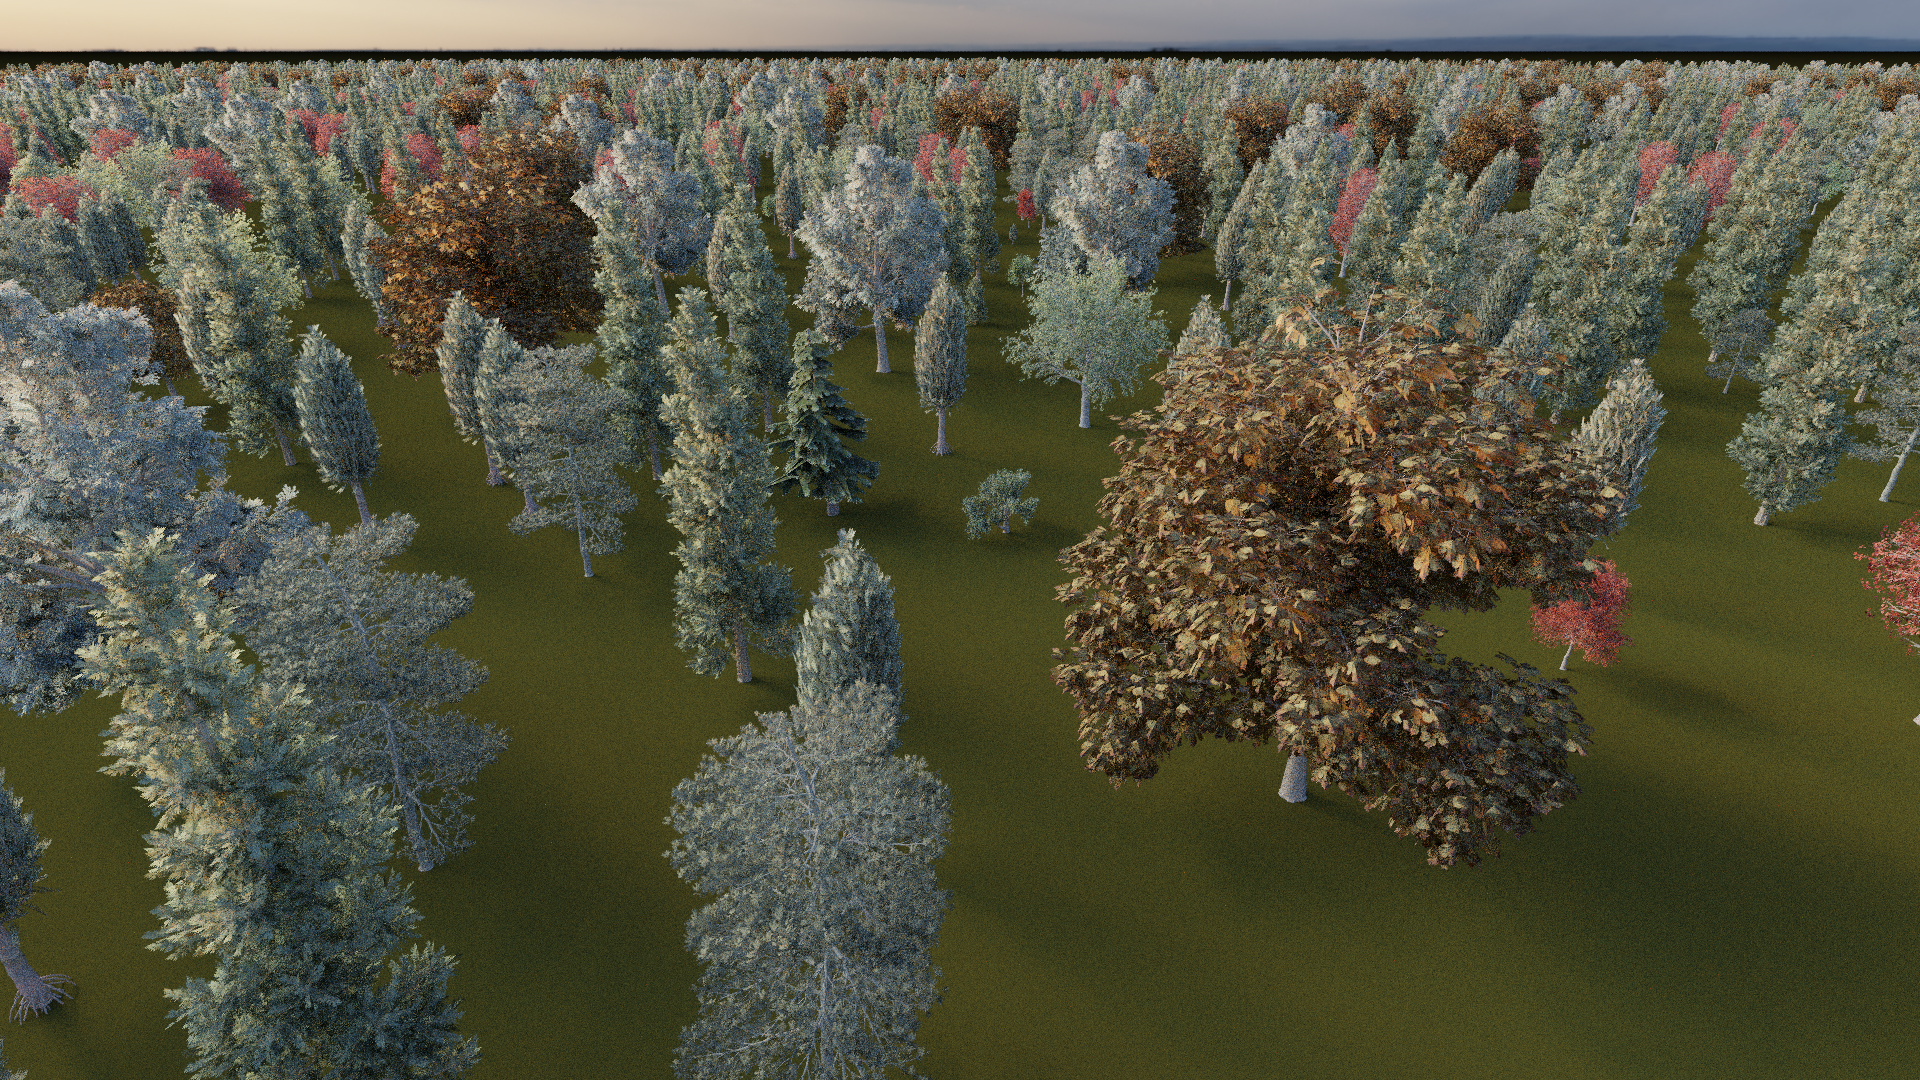
\includegraphics[width=1\linewidth]{img/results/diffuse_only_mesh.jpg}
        \caption{}
        % \label{fig:render_comparison_mesh}
    \end{subfigure}
    \begin{subfigure}[b]{0.49\linewidth}
        \centering
        \includegraphics[width=1\linewidth]{img/results/specular_only_mesh.jpg}
        \caption{}
        % \label{fig:render_comparison_lod}
    \end{subfigure}
    \begin{subfigure}[b]{0.49\linewidth}
        \centering
        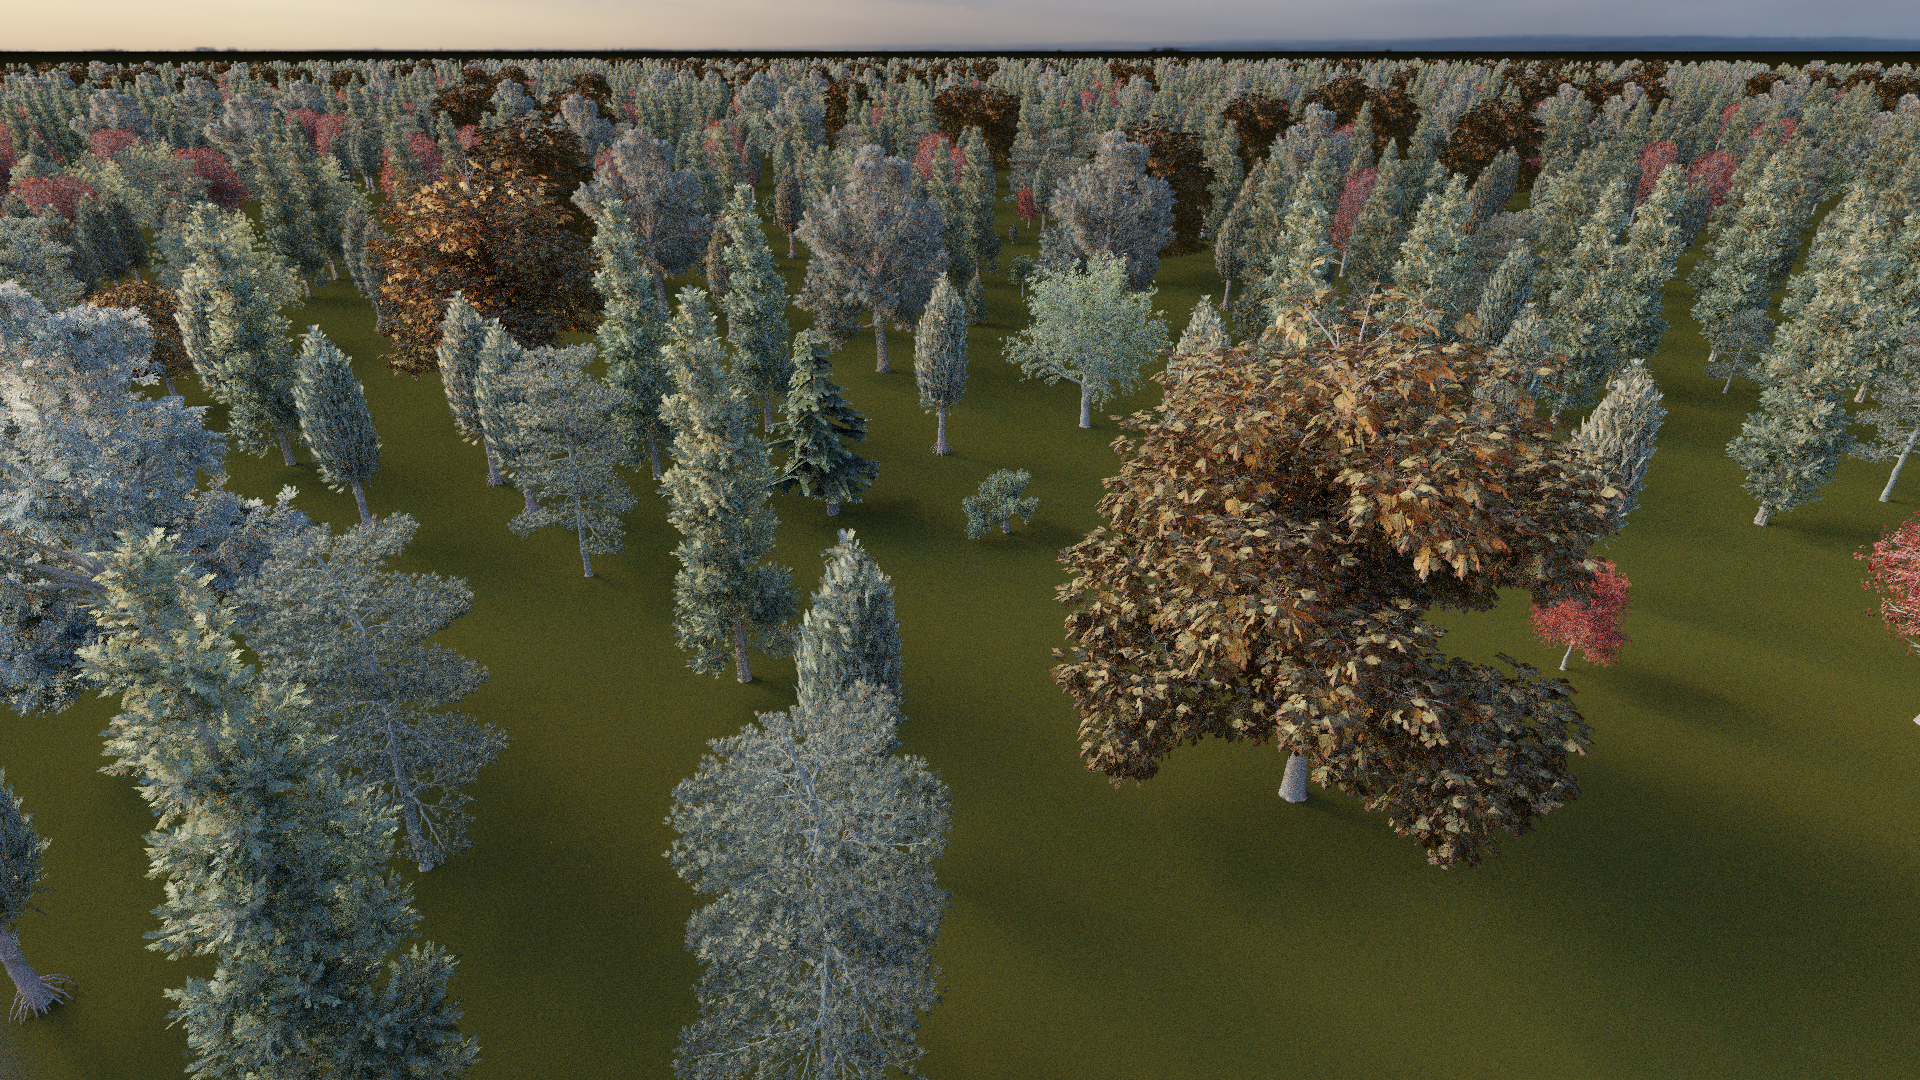
\includegraphics[width=1\linewidth]{img/results/diffuse_only_lod_1A.jpg}
        \caption{}
        % \label{fig:render_comparison_mesh}
    \end{subfigure}
    \begin{subfigure}[b]{0.49\linewidth}
        \centering
        \includegraphics[width=1\linewidth]{img/results/specular_only_lod_1A.jpg}
        \caption{}
        % \label{fig:render_comparison_lod}
    \end{subfigure}
    % \caption[Comparison between mesh and volume renderings of the forest]{Renderings of the forest using meshes only (a) and using \acsp{lod} if a voxel is smaller than a pixel (b).}
    \caption[Diffuse and specular components rendered seperately]{(a) and (b) show the diffuse respectively specular component of the reference image, (c) and (d) show the diffuse respectively specular component when using \acsp{lod} where a voxel covers at most one pixel. The images are rendered with 32 samples per pixel.}
	\label{fig:diffuse_specular_breakdown}
\end{figure}
In the volumes the diffuse phase function gives way more uniform looking trees without these bright regions on the sun-facing side.
The specular component gives discrete specular highlights on the surfaces while the specular phase function leads to reflections across the whole medium.
So obviously our approach fails in preserving the visual appearance of the meshes.
We identify two reasons for this limitation: First, the \ac{sggx} phase function is defined on the whole unit sphere (recall Figure \ref{fig:sggx_ndf}), which means that half of the rays are reflected into the medium where they are attenuated, while for surfaces all rays are reflected away from the surface.
Second, it is likely that this error is due to the usage of an isotropic microflake projected area, which directly influences our density values.
As we showed in Section \ref{sec:mesh_filtering} the optimization of the density depends on this projected area and by choosing a constant value we ignore for example how the roughness of a material influences the density.
Rising roughness values therefore lead to decreasing density values, since $P_{occ}$ from Equation \ref{eq:our_filtering_equation} decreases.
This can lead to a significantly different look because the rays scatter earlier.
The filtering procedure however, would become more complex.
Experiments in this direction are outside of the scope of this thesis.

% This affects our density values, since the density is also optimized based on the microflake projected area $sigma$.
%  which effectively leads to reflection directions that are uniformly scattered on the unit sphere.
% % Second, it is likely that this error is due to the usage of an isotropic extinction coefficient, which effectively leads to reflection directions that are uniformly scattered on the unit sphere.
% Therefore we could reduce the error by using an anisotropic extinction, which would lead to a more complex filtering procedure.

Apart from these visual problems, the render time for the \ac{lod} approach is another concern.
The duration is currently with $\SI{8723}{\s}$ for 1024 samples per pixel (Figure \ref{fig:render_comparison_lod}) slower than rendering only the meshes, which took $\SI{5463}{\s}$ for 1024 samples per pixel (Figure \ref{fig:render_comparison_mesh}).
As we just discussed, we recognize the \acsp{lod} mainly by their different color and not by their details or blurriness.
We therefore have some room left for tweaking the distance at which we switch to \ac{lod} rendering or we can use coarser \acsp{lod}.
Tweaking the distance translates to changing the number of pixels a voxel may cover.
As we wrote in Section \ref{sec:scene_generation} our heuristic currently ensures that a voxel covers at most one pixel.
Now we relax this restriction and measure render times when a voxel covers 1, 4, 9 or 16 pixels.
Additionally we test how changing the voxel size of the finest \ac{lod} affects performance.
Before, the voxels in our finest \ac{lod} had a size of 0.1m.
Now we choose a minimal voxel size of 0.1m, 0.2m, 0.4m, 0.8m, 1.6m, 3.2m and 6.4m.
In total this gives us 28 combinations that we have to test.
% We visualize our measurements in Figure \ref{fig:render_durations} as a heat map.
In Figure \ref{fig:lod_grid} we visualize the durations as well as the \FLIP error for rendering the different configurations with 32 samples per pixel.
\begin{figure}[ht]
    \centering
    \begin{subfigure}[b]{0.49\linewidth}
        \centering
        \includegraphics[width=1\linewidth]{img/results/render_durations.png}
        \caption{}
    \end{subfigure}
    \begin{subfigure}[b]{0.49\linewidth}
        \centering
        \includegraphics[width=1\linewidth]{img/results/flip_errors.png}
        \caption{}
    \end{subfigure}
	\caption[Heatmap of the \ac{lod} render durations and \FLIP errors.]{Heatmap for render durations (a) and the mean \FLIP error (b) of different combinations of the minimum voxel size and the number of covered pixels. Bright regions indicate high values, dark regions indicate low values.}
	\label{fig:lod_grid}
\end{figure}
We can see that when we start \ac{lod} rendering with rougher \acsp{lod} we can reduce rendertimes to a certain degree before they rise again.
The decline happens because rougher \acsp{lod} are less memory intensive then the fine \acsp{lod} and therefore easier to cache.
At the same time increasing the minimum voxel size for a fixed number of covered pixels pushes the boundary of the \ac{lod} switch away from the camera which increases the number of meshes to be rendered.
The meshes take longer to render than the rough \acsp{lod}, therefore the render time increases again.

We get another view on the different combinations between the number of covered pixels and the minimum voxel size if we visualize the bounding boxes, like we previously did in Figure \ref{fig:visualize_lods}.
Now we not only show a rendering from above the scene but also from the main camera perspective.
Figure \ref{fig:visualize_lods_different_configurations_covered_pixels_fixed} visualizes the previously described effect, that increasing the minimum voxel size with a fixed number of covered pixels increases the distance at which \acsp{lod} are rendered.
\begin{figure}
    \begin{subfigure}[b]{\linewidth}
        \begin{center}
            \begin{tabular}{ c c c c  }
                \adjustimage{width=0.22\textwidth,valign=m}{img/results/visualize_lods_1A_front.jpg} & \adjustimage{width=0.22\textwidth,valign=m}{img/results/visualize_lods_1B_front.jpg} & \adjustimage{width=0.22\textwidth,valign=m}{img/results/visualize_lods_1C_front.jpg} & \adjustimage{width=0.22\textwidth,valign=m}{img/results/visualize_lods_1D_front.jpg} \\
                \adjustimage{width=0.22\textwidth,valign=m}{img/results/visualize_lods_1A_top.jpg} & \adjustimage{width=0.22\textwidth,valign=m}{img/results/visualize_lods_1B_top.jpg} & \adjustimage{width=0.22\textwidth,valign=m}{img/results/visualize_lods_1C_top.jpg} & \adjustimage{width=0.22\textwidth,valign=m}{img/results/visualize_lods_1D_top.jpg} \\
                {\footnotesize Covered pixels = 1} & {\footnotesize Covered pixels = 4} & {\footnotesize Covered pixels = 9} & {\footnotesize Covered pixels = 16} \\
            \end{tabular}
        \end{center}
        \caption{}
        \label{fig:visualize_lods_different_configurations_min_voxel_size_fixed}
    \end{subfigure}
    \begin{subfigure}[b]{\linewidth}
        \begin{center}
            \begin{tabular}{ c c c c  }
                \adjustimage{width=0.22\textwidth,valign=m}{img/results/visualize_lods_1A_front.jpg} & \adjustimage{width=0.22\textwidth,valign=m}{img/results/visualize_lods_2A_front.jpg} & \adjustimage{width=0.22\textwidth,valign=m}{img/results/visualize_lods_3A_front.jpg} & \adjustimage{width=0.22\textwidth,valign=m}{img/results/visualize_lods_4A_front.jpg} \\
                \adjustimage{width=0.22\textwidth,valign=m}{img/results/visualize_lods_1A_top.jpg} & \adjustimage{width=0.22\textwidth,valign=m}{img/results/visualize_lods_2A_top.jpg} & \adjustimage{width=0.22\textwidth,valign=m}{img/results/visualize_lods_3A_top.jpg} & \adjustimage{width=0.22\textwidth,valign=m}{img/results/visualize_lods_4A_top.jpg} \\
                % Covered pixels = 1 & Covered pixels = 4 & Covered pixels = 9 & Covered pixels = 16 \\
                {\footnotesize Min. voxel size = $\SI{0.1}{\m}$} & {\footnotesize Min. voxel size = $\SI{0.2}{\m}$} & {\footnotesize Min. voxel size = $\SI{0.4}{\m}$} & {\footnotesize Min.\newline voxel size = $\SI{0.8}{\m}$}\\
            \end{tabular}
        \end{center}
        \caption{}
        \label{fig:visualize_lods_different_configurations_covered_pixels_fixed}
    \end{subfigure}
    \caption[Visualization of \acsp{lod} using different configurations]{Debug views of the volume bounding boxes for different configurations. In (a) the minimum voxel size is fixed at $\SI{0.1}{\m}$ and we vary the number of covered pixels, while in (b) the number of covered pixels is fixed at 1 and we vary the minimum voxel size. Blue is again the finest \ac{lod} and red the coarsest \ac{lod}. }
    \label{fig:visualize_lods_different_configurations}
\end{figure}
For the case of a fixed number of covered pixels and a minimum voxel size of $\SI{0.8}{\m}$ it is also interesting to note that the distance based \acsp{lod} still cover almost half of the circular forest, although they are barely visible from the main camera's perspective.


% We get another view on the increasing distances of \ac{lod} rendering when we look at the colored bounding boxes of the volumes again ...
Looking back at Figure \ref{fig:lod_grid}, the influence of the memory footprint of a grid on the render performance becomes especially apparent at a minimum voxel size of 0.1m, where we observe almost a doubling of the render time between our default combination with one covered pixel per voxel and when up to 16 pixels may be covered.
Overall the best result is achieved by dropping the three finest \acsp{lod} and let each voxel cover up to four pixels.
The scene then renders in 179s which is a 27\% improvement over rendering only meshes.
Additionally it has the positive side-effect that the shading problem is less noticeable, which is reflected in a drop in the mean \FLIP error from 0.123 to 0.096.
Figure \ref{fig:render_and_error_fastest} shows this rendering with the corresponding \FLIP error map.
\begin{figure}[ht]
    \centering
    \begin{subfigure}[b]{0.9\linewidth}
        \centering
        \includegraphics[width=1\linewidth]{img/results/rendering_lod_4B.jpg}
        \caption{}
    \end{subfigure}
    \begin{subfigure}[b]{0.9\linewidth}
        \centering
        \includegraphics[width=1\linewidth]{img/results/flip_error_4B.jpg}
        \caption{}
    \end{subfigure}
    \caption[Rendering and \FLIP error map of the fastest combination]{(a) shows the fastest rendering, finished in 179s for 32 samples. The scene is generated with a minimum voxel size of 0.8m and up to four covered pixels per voxel. (b) shows the corresponding \FLIP error map against the ground truth. The mean \FLIP error is 0.096.}
    \label{fig:render_and_error_fastest}
\end{figure}
We can further decrease the mean \FLIP error down to 0.088, for example by choosing a minimum voxel size of 6.4 meters and let each voxel cover one pixel, at the cost of a higher render time.
The rendering with the lowest \FLIP error is visually indistinguishable from the ground truth rendering.


Actually meshes can also render faster than rough \acsp{lod}, when taking the distance into account.
When we look at \ref{fig:render_time_comparisons}, we see that all \acsp{lod} initially render slower than the mesh representations.
\begin{figure}[ht]
    \centering
    \begin{subfigure}[b]{0.49\linewidth}
        \centering
        \includegraphics[width=1\linewidth]{img/results/render_durations_PR04a.png}
        \caption{}
    \end{subfigure}
    \begin{subfigure}[b]{0.49\linewidth}
        \centering
        \includegraphics[width=1\linewidth]{img/results/render_durations_EA01a.png}
        \caption{}
    \end{subfigure}
	\caption[Plots of the render times depending on the distance from the camera.]{These plots show the render times depending on the distance from the camera for single instances of the model \textit{Asterophyllites equisetiformis adult} (a) and for \textit{Acer rubrum adult} (b). Meshes render faster than all \acsp{lod} until a certain distance.}
	\label{fig:render_time_comparisons}
\end{figure}
However their render times fall rapidly with the distance until they eventually are below the mesh render time.
It is interesting to note, that the mesh render time first also declines slightly before it rises steadily.
An explanation for this can be that at a certain distance the random sampling of a pixel produces large jumps across the bounding volume hierarchy, which leads to many cache misses.








\chapter{Future Work}
\label{chap:future_work}
As we discovered, the abilities of our approach to preserve the look of the surface mesh is not satisfactory.
The next step to improve on this would be to include anisotropic extinction, which would require a rewrite of the filtering procedure and the distance sampling and transmittance estimation.
The existing volumes would not be compatible with this new approach and had to be re-generated as well.

To further enhance the quality of the renderings, it would be interesting how our volumetric \ac{lod} approach performs with spectral rendering.
This would improve physical accuracy since the scattering in media is actually wavelength dependent \cite{novak_overview} but it requires a rewrite of the renderer.
Since this increases the dimension of the rendering equation it leads to an increase in the render duration and is currently only feasible for offline rendering.
A performance improvement should still be the result.

Another interesting area of research would be to further improve the performance of our approach and possibly switch the \acsp{lod} on the fly.
This would allow a camera movement without making the \acsp{lod} misalign the current view frustum.
The scene generator would have to be written in C++ for that and optimization of the program itself have to be made.
A large improvement can be expected by caching the free positions in the forest area, since we initialize the random number generator with the same seed anyway.
However this is limited to our forest scene.
A more portable optimization would be to approximate the pixels a bounding box covers by a rectangle instead of the convex hull that we currently use.
Also using brick grid for storing all voxel attributes like color values or the \ac{sggx} matrix $S$ might be worth investigating regarding the performance implications.

Having the knowledge that rough \acsp{lod} do not necessarily render faster than meshes, a further optimization would be to not simply set models outside of the view frustum to the roughest \ac{lod}.
Instead it might be beneficial to also incorporate the distance to the camera for these and use the mesh representations first.
Only after a certain distance from the camera the roughest \ac{lod} would be selected.
Furthermore, we might want to use a different heuristic of \ac{lod} selection for each model, since we learned from Figure \ref{fig:render_time_comparisons} that \ac{lod} rendering surpasses mesh rendering at different distances for different models.

\chapter{Summary}
\label{chap:summary}
This thesis presented an approach for filtering textured surface meshes, thereby converting them into volumes.
The resulting volumetric representations occupy 22\% less disk space.
We further developed a scene generator that uniformly distributes models on a circular area.
It selects an appropriate \ac{lod} based on the number of pixels that a volume covers compared to the number of voxels visible from the camera.
We then rendered a scene containing only meshes and scenes with different \ac{lod} selection strategies in our custom physically based path tracer.
We find that we can decrease render times by up to 17\% while introducing a \FLIP error of 0.038.
Lower \FLIP errors are possible at the cost of higher render times.
We can therefore conclude that volumetric representations of surface meshes can reduce rendertimes while introducing noticeable differences in the image quality in a side by side comparison.

% ---------- Anhang ----------

\begin{appendix}
	% \chapter[Appendix]{}

\chapter{\acs{psnr} and \acs{ssim} Image Errors}
\label{chap:psnr_and_ssim_errors}

\section{Forest Scene}
In the following we provide the \ac{psnr} and \ac{ssim} errors for the different combinations between the number of covered pixels and the minimum \ac{lod} size.

The \ac{psnr} values (in dB) are:
\begin{center}
    \begin{tabular}{| c | c | c | c | c | c | c | c | c |}
        \cline{3-9}
        \multicolumn{2}{c|}{} & \multicolumn{7}{c|}{Minimum voxel size [m]} \\
        \cline{3-9}
        \multicolumn{2}{c|}{} & 0.1 & 0.2 & 0.4 & 0.8 & 1.6 & 3.2 & 6.4 \\
        \hline
        \multirow{4}{*}{Covered pixels}& 1 & 29.0 & 31.8 & 34.7 & 36.4 & 37.3 & 37.3 & 37.3 \\
        \cline{2-9}
        & 4 & 26.5 & 28.6 & 31.2 & 34.0 & 36.0 & 37.2 & 37.3 \\
        \cline{2-9}
        & 9 & 23.0 & 26.4 & 29.3 & 31.7 & 34.3 & 36.4 & 37.3 \\
        \cline{2-9}
        & 16 & 22.6 & 25.6 & 27.6 & 30.0 & 33.0 & 35.3 & 36.9 \\
        \hline
    \end{tabular}
\end{center}

The \ac{ssim} values are:
\begin{center}
    \begin{tabular}{| c | c | c | c | c | c | c | c | c |}
        \cline{3-9}
        \multicolumn{2}{c|}{} & \multicolumn{7}{c|}{Minimum voxel size [m]} \\
        \cline{3-9}
        \multicolumn{2}{c|}{} & 0.1 & 0.2 & 0.4 & 0.8 & 1.6 & 3.2 & 6.4 \\
        \hline
        \multirow{4}{*}{Covered pixels}& 1 & 0.905 & 0.941 & 0.960 & 0.967 & 0.970 & 0.970 & 0.970 \\
        \cline{2-9}
        & 4 & 0.828 & 0.887 & 0.932 & 0.956 & 0.966 & 0.969 & 0.970 \\
        \cline{2-9}
        & 9 & 0.682 & 0.819 & 0.900 & 0.938 & 0.958 & 0.967 & 0.970 \\
        \cline{2-9}
        & 16 & 0.637 & 0.784 & 0.858 & 0.917 & 0.951 & 0.963 & 0.969 \\
        \hline
    \end{tabular}
\end{center}

% \newpage
\section{Single Instance Renderings}
We also provide the \ac{psnr} and \ac{ssim} errors for the single instance renderings in the following.

\textit{Celtis australis adult}:
\begin{center}
    \begin{tabular}{| c | c | c | c | c | c | c | c |}
        \cline{2-8}
        \multicolumn{1}{c|}{} & \multicolumn{7}{c|}{Voxel size [m]} \\
        \cline{2-8}
        \multicolumn{1}{c|}{} & 0.1 & 0.2 & 0.4 & 0.8 & 1.6 & 3.2 & 6.4 \\
        \hline
        Duration [s] & 805 & 522 & 376 & 304 & 218 & 201 & 179 \\
        \hline
        \acs{psnr} [dB] & 24.2 & 23.5 & 22.9 & 22.2 & 21.7 & 21.1 & 20.0 \\
        \hline
        \acs{ssim} & 0.718 & 0.677 & 0.663 & 0.657 & 0.655 & 0.650 & 0.642 \\
        \hline
    \end{tabular}
\end{center}

\textit{Acer rubrum adult}:
\begin{center}
    \begin{tabular}{| c | c | c | c | c | c | c | c |}
        \cline{2-8}
        \multicolumn{1}{c|}{} & \multicolumn{7}{c|}{Voxel size [m]} \\
        \cline{2-8}
        \multicolumn{1}{c|}{} & 0.1 & 0.2 & 0.4 & 0.8 & 1.6 & 3.2 & 6.4 \\
        \hline
        Duration [s] & 685 & 453 & 335 & 279 & 217 & 205 & 194 \\
        \hline
        \acs{psnr} [dB] & 21.0 & 20.6 & 20.2 & 19.9 & 19.3 & 18.6 & 17.8 \\
        \hline
        \acs{ssim} & 0.636 & 0.585 & 0.571 & 0.566 & 0.561 & 0.556 & 0.540 \\
        \hline
    \end{tabular}
\end{center}
\end{appendix}

% ---------- Verzeichnisse ----------

\listoffigures
%\listoftables
%\lstlistoflistings

% ----------------------------

% Erzeugt das Literaturverzeichnis
\printbibliography

% Erzeugt eine Seite mit der Erklaerung
\declaration{nutzung}

\end{document}
